\documentclass[
11pt, % The default document font size, options: 10pt, 11pt, 12pt
codirector, % Uncomment to add a codirector to the title page
]{plan} 




% El títulos de la memoria, se usa en la carátula y se puede usar el cualquier lugar del documento con el comando \ttitle
\titulo{Cámara de seguridad IoT con conectividad LoRaWAN} 

% Nombre del posgrado, se usa en la carátula y se puede usar el cualquier lugar del documento con el comando \degreename
%\posgrado{Carrera de Especialización en Sistemas Embebidos} 
%\posgrado{Carrera de Especialización en Internet de las Cosas} 
%\posgrado{Carrera de Especialización en Intelegencia Artificial}
\posgrado{Maestría en Sistemas Embebidos} 
%\posgrado{Maestría en Internet de las cosas}

% Tu nombre, se puede usar el cualquier lugar del documento con el comando \authorname
\autor{Esp. Ing. Mauricio Barroso Benavides} 

% El nombre del director y co-director, se puede usar el cualquier lugar del documento con el comando \supname y \cosupname y \pertesupname y \pertecosupname
\director{Mg. Ing. Gonzalo Sanchez}
\pertenenciaDirector{
FF.AA, FIUBA} 
% FIXME:NO IMPLEMENTADO EL CODIRECTOR ni su pertenencia
\codirector{John Doe} % para que aparezca en la portada se debe descomentar la opción codirector en el documentclass
\pertenenciaCoDirector{FIUBA}

% Nombre del cliente, quien va a aprobar los resultados del proyecto, se puede usar con el comando \clientename y \empclientename
\cliente{Nombre del cliente}
\empresaCliente{Empresa del cliente}

% Nombre y pertenencia de los jurados, se pueden usar el cualquier lugar del documento con el comando \jurunoname, \jurdosname y \jurtresname y \perteunoname, \pertedosname y \pertetresname.
\juradoUno{Nombre y Apellido (1)}
\pertenenciaJurUno{pertenencia (1)} 
\juradoDos{Nombre y Apellido (2)}
\pertenenciaJurDos{pertenencia (2)}
\juradoTres{Nombre y Apellido (3)}
\pertenenciaJurTres{pertenencia (3)}
 
\fechaINICIO{23 de junio de 2021}		%Fecha de inicio de la cursada de GdP \fechaInicioName
\fechaFINALPlan{11 de agosto de 2021} 	%Fecha de final de cursada de GdP
\fechaFINALTrabajo{15 de mayo de 2022}	%Fecha de defensa pública del trabajo final


\begin{document}

\maketitle
\thispagestyle{empty}
\pagebreak


\thispagestyle{empty}
{\setlength{\parskip}{0pt}
\tableofcontents{}
}
\pagebreak


\section*{Registros de cambios}
\label{sec:registro}


\begin{table}[ht]
\label{tab:registro}
\centering
\begin{tabularx}{\linewidth}{@{}|c|X|c|@{}}
\hline
\rowcolor[HTML]{C0C0C0} 
Revisión & \multicolumn{1}{c|}{\cellcolor[HTML]{C0C0C0}Detalles de los cambios realizados} & Fecha      \\ \hline
0      & Creación del documento                                 &\fechaInicioName \\ \hline
1      & Se completa hasta el punto 5 inclusive                 & 13 de julio de 2021 \\
 \hline
2      & Se completa hasta el punto 9 inclusive                 & 27 de julio de 2021 \\
 \hline
% 2      & Se completa hasta el punto 9 inclusive                 & 27 de julio de 2021 \\ \hline
%2      & Se completa hasta el punto 7 inclusive
%		  Se puede agregar algo más \newline
%		  En distintas líneas \newline
%		  Así                                                    & dd/mm/aaaa \\ \hline
%3      & Se completa hasta el punto 11 inclusive                & dd/mm/aaaa \\ \hline
%4      & Se completa el plan	                                 & dd/mm/aaaa \\ \hline
\end{tabularx}
\end{table}

\pagebreak



\section*{Acta de constitución del proyecto}
\label{sec:acta}

\begin{flushright}
Buenos Aires, \fechaInicioName
\end{flushright}

\vspace{2cm}

Por medio de la presente se acuerda con el \authorname\hspace{1px} que su Trabajo Final de la \degreename\hspace{1px} se titulará ``\ttitle'', consistirá esencialmente en la implementación de un prototipo de una cámara de seguridad para entornos IoT con conectividad LoRaWAN, y tendrá un presupuesto preliminar estimado de 600 hs de trabajo y US\$200, con fecha de inicio \fechaInicioName\hspace{1px} y fecha de presentación pública \fechaFinalName.

Se adjunta a esta acta la planificación inicial.

\vfill

% Esta parte se construye sola con la información que hayan cargado en el preámbulo del documento y no debe modificarla
\begin{table}[ht]
\centering
\begin{tabular}{ccc}
\begin{tabular}[c]{@{}c@{}}Ariel Lutenberg \\ Director posgrado FIUBA\end{tabular} & \hspace{2cm} & \begin{tabular}[c]{@{}c@{}}\supname \\ Director del Trabajo Final\end{tabular} \vspace{2.5cm} \\ 
%\multicolumn{3}{c}{\begin{tabular}[c]{@{}c@{}} \supname \\ Director del Trabajo Final\end{tabular}} \vspace{2.5cm} \\
%\begin{tabular}[c]{@{}c@{}}\jurunoname \\ Jurado del Trabajo Final\end{tabular}     &  & \begin{tabular}[c]{@{}c@{}}\jurdosname\\ Jurado del Trabajo Final\end{tabular}  \vspace{2.5cm}  \\
%\multicolumn{3}{c}{\begin{tabular}[c]{@{}c@{}} \jurtresname\\ Jurado del Trabajo Final\end{tabular}} \vspace{.5cm}                                                                     
\end{tabular}
\end{table}




\section{1. Descripción técnica-conceptual del proyecto a realizar}
\label{sec:descripcion}

La seguridad de espacios y bienes es un aspecto muy importante en la vida de las personas. Es así que en el mercado existen distintos tipos de soluciones basadas en dispositivos electrónicos, que permiten controlar y monitorear los espacios geográficos en donde se encuentran instalados. Estos dispositivos en conjunto forman sistemas de seguridad, que pueden detectar mediante distintos tipos de datos eventos no deseados.

Los dispositivos electrónicos de seguridad más utilizados son las cámaras. Estas permiten obtener imágenes en forma de videos o fotografías del sector en particular donde se encuentran. Los primeros sistemas de seguridad basados en cámaras necesitaban de un dispositivo para almacenar las imágenes que obtenían. Hoy en día las cámaras de seguridad poseen distintos tipos de conectividad hacia Internet, lo que les permite transmitir las imágenes que obtienen hacia servidores en la nube para que sean procesadas y almacenadas.

La transferencia de datos desde una cámara de seguridad hacia Internet requiere de un gran ancho de banda, por lo que es muy común que estos dispositivos posean conectividad Wi-Fi (inalámbrico) y/o Ethernet (cableado). La utilización de estas conexiones implica la existencia previa de, generalmente, una red de tipo LAN (Local Area Network) que consta principalmente de un router que se encarga de proporcionar direciones IP (Internet Protocol) a todos los dispositivos de la red. Este escenario es muy común en entornos urbanos, donde, los proveedores de Internet proporcionan a sus usuarios conexiones estables y de gran ancho de banda, a través de redes de fibra óptica y/o cable coaxial.

Por otro lado, las zonas rurales no cuentan con la cobertura de los proveedores de Internet de las zonas urbanas, ya que a estos no les resulta rentable, y en muchos casos posible, instalar toda la infraestructura necesaria para proporcionar sus servicios. Para estos casos existen cámaras de seguridad con conectividad móvil (redes de telefonía) para transferir datos hacia Internet. Aunque esto supone un costo económico adicional que varía en función de la cantidad de datos transferidos, es una de las pocas soluciones viables que existen actualmente en el mercado. Es común también que este tipo de cámaras dispongan de una fuente de alimentación basada en baterías o paneles solares.

Entonces, el objetivo de este trabajo es diseñar e implementar una cámara de seguridad que pueda utilizarse en lugares donde no existen redes de banda ancha y tampoco una fuente de alimentación constante, y de esta manera lograr un dispositivo con la capacidad solucionar la problemática de planteada previamente.

El desarrollo de este proyecto está basado principalmente en el área de sistemas embebidos, pero también incorpora elementos propios de IoT (Internet of Things) y ML (Machine Learning) para lograr prestaciones adecuadas al contexto actual. El Internet de las cosas o IoT, por sus siglas en inglés, se refiere a la conexión de dispositivos y objetos a Internet con el objetivo de monitorearlos e interactuar con ellos de manera remota. IoT plantea algunas problemáticas como la seguridad de la información, la alimentación de dispositivos que no disponen de una fuente de energía eléctrica constante y la administración del ancho de banda disponible. El aprendizaje automático o ML, por sus siglas en inglés, permite a los sistemas computacionales realizar predicciones y tomar decisiones en función de los datos de entrada. En los últimos años la optimización que han tenido los algoritmos de ML permiten que estos puedan ser ejecutados en sistemas embebidos, lo que da como resultado una amplia gama de nuevas aplicaciones y otra perspectiva para resolver problemas antes planteados.

Dentro de un entorno IoT elegir el tipo de red para la interconexión de nodos finales con Internet es un aspecto muy importante. Es así que, en aplicaciones donde el consumo energético y el aprovechamiento de ancho de banda son importantes, LoRaWAN es el tipo de red óptimo para estos casos. Esta red permite la conexión de nodos finales hacía gateways conectados a Internet hasta una distancia teórica de 20 Km y con un ancho de banda de hasta 500 KHz (US915). La topología de red a utilizar en este proyecto sería la que observa en la figura \ref{fig:topology}.

\begin{figure}[htpb]
\centering 
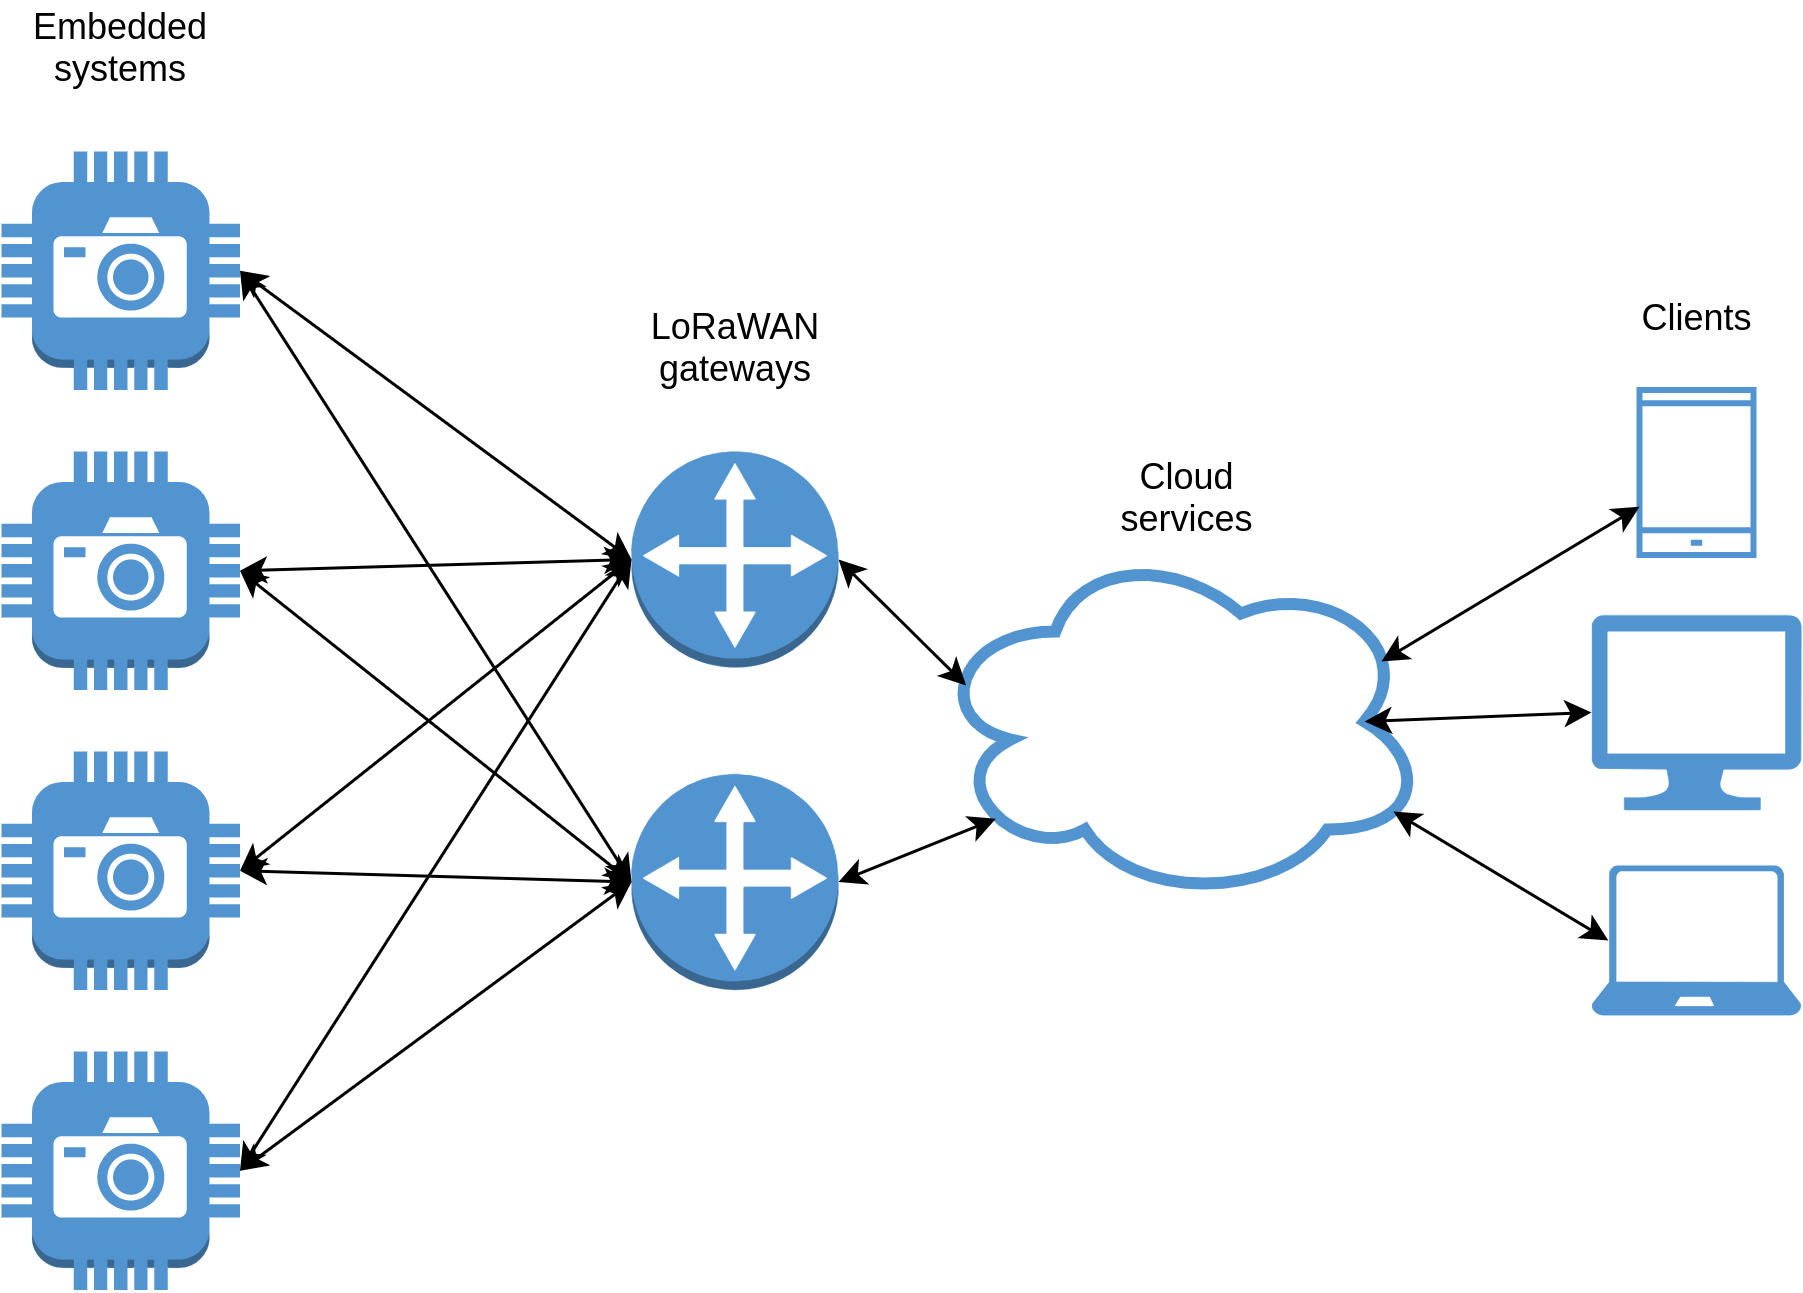
\includegraphics[width=0.8\textwidth]{./fig/topology.png}
\caption{Diagrama en bloques del sistema}
\label{fig:topology}
\end{figure}

\vspace{25px}

Según todas las características antes descritas, el sistema embebido implicado en este trabajo deberá tener el diagrama de bloques que se expone en la figura \ref{fig:blocks}.

\begin{figure}[htpb]
\centering 
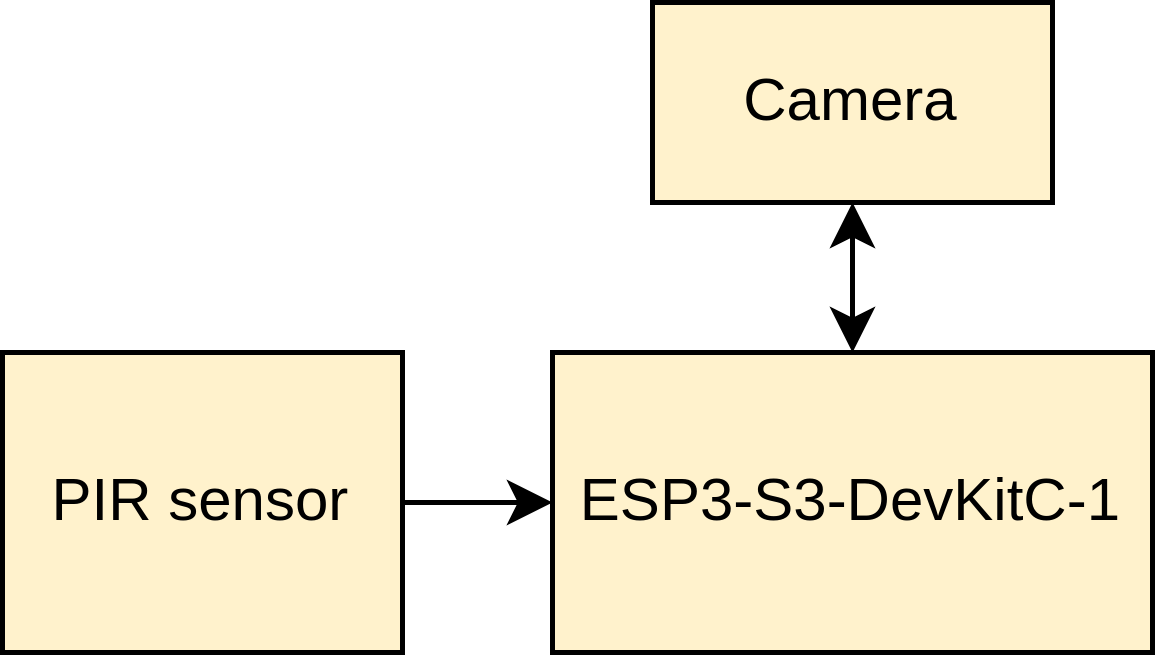
\includegraphics[width=0.5\textwidth]{./fig/blocks.png}
\caption{Diagrama en bloques del sistema}
\label{fig:blocks}
\end{figure}

\vspace{25px}

El sistema embebido tiene como componente más importante un microcontrolador que se encarga principalmente de ejecutar un modelo de machine learning para la detección de personas, sus entradas son los valores leídos por la cámara y el sensor de movimiento PIR (Passive InfraRed). Otra función del microcontrolador es la ejecución del stack LoRaWAN, para que en conjunto con el transceptor LoRa, el sistema pueda interactuar correctamente dentro de una red de este tipo. Finalmente, se cuenta con una tarjeta SD (Secure Digital) para almacenar las imágenes capturadas por la cámara.

\section{2. Identificación y análisis de los interesados}
\label{sec:interesados}

\begin{table}[ht]
%\caption{Identificación de los interesados}
%\label{tab:interesados}
\begin{tabularx}{\linewidth}{@{}|l|X|X|l|@{}}
\hline
\rowcolor[HTML]{C0C0C0} 
Rol           & Nombre y Apellido & Organización 			& Puesto 	\\ \hline
Responsable   & \authorname		& -        				& Alumno 	\\ \hline
Orientador    & \supname			& - 						& Director Trabajo final \\ \hline
Usuario final & -                 & -             			& -       	\\ \hline
\end{tabularx}
\end{table}

\begin{itemize}
	\item Orientador: Tiene la capacidad de ayudar al alumno a resolver los problemas técnicos y conceptuales que se presenten a lo largo del proyecto. Es exigente con los tiempos y la calidad del desarrollo del proyecto.
	\item Usuario final: No posee conocimientos sobre sistemas embebidos y las tecnologías utilizadas en el proyecto, y espera dispositivos de bajo costo económico.
\end{itemize}



\section{3. Propósito del proyecto}
\label{sec:proposito}

El propósito de este proyecto es diseñar e implementar un sistema embebido que funcione como cáma de seguridad en un entorno IoT con ayuda de algoritmos de ML. 

Un propósito personal del autor es obtener conocimientos y experiencia sobre implementación de algoritmos de ML en sistemas embebidos.

\section{4. Alcance del proyecto}
\label{sec:alcance}

Este proyecto incluye:
\begin{itemize}
	\item Diseño e implementación del firmware del sistema embebido.
	\item Diseño e implementación del algoritmo de ML para reconocimiento de personas.
	\item Implementación del sistema embebido desarrollado dentro de una arquitectura IoT existente.
	\item Diseño del PCB para el prototipo funcional del sistema embebido.
	\item Creación de documentación sobre datos técnicos y características del sistema embebido.
\end{itemize}

Este proyecto no incluye:
\begin{itemize}
	\item Implementación del PCB para el prototipo funcional del sistema embebido.
	\item Desarrollo de una aplicación para el usuario final.
\end{itemize}

\section{5. Supuestos del proyecto}
\label{sec:supuestos}

\begin{itemize}
	\item Se contará con el presupuesto necesario para obtener los componentes del proyecto.
	\item Se dedicarán al menos 2 horas diarias para la realización del proyecto.
	\item Se dispondrá de una arquitectura IoT para redes LoRaWAN para la realización de pruebas y puesta en marcha del proyecto.
\end{itemize}

\section{6. Requerimientos}
\label{sec:requerimientos}

El presente proyecto tiene dos tipos de requerimientos, funcionales y no funcionales. A continuación se citan los antes referidos.

\begin{enumerate}
	\item Requerimientos funcionales
		\begin{enumerate}
			\item El sistema debe conectarse a una red LoRaWAN en la banda de frecuencia AU915 como dispositivo de clase A.
			\item El sistema debe ser alimentado mediante dos baterías de tipo AA.
			\item El sistema debe poseer mecanismos de seguridad implementados tanto en hardware como en software para evitar su manipulación incorrecta.
			\item El sistema debe almacenar fotografías y videos obtenidos mediante su cámara cámara en una memoria no volátil.
			\item El sistema debe recibir su configuración inicial mediante interruptores físicos conectados al mismo.
			\item El sistema debe recibir sus parámetros de funcionamiento mediante la red LoRaWAN a la que esta conectada.
			\item El sistema debe funcionar solamente si se detecta movimiento en el sector donde se encuentra instalada.
			\item El sistema debe ser compatible con la especificación LoRaWAN 1.0.2.
			\item El ssitema debe, con ayuda de su cámara, detectar la presencia de personas a través de un algorito de ML.
		\end{enumerate}
	\item Requerimientos no funcionales
		\begin{enumerate}
			\item El sistema deberá tener un costo de desarrollo igual o menor a 200\$us.
			\item El sistema deberá tener documentación adecuada sobre su uso y desarrollo.
		\end{enumerate}
\end{enumerate}

\section{7. Historias de usuarios (\textit{Product backlog})}
\label{sec:backlog}

El criterio para determinar los \textit{storyboards} es el siguiente.

\begin{itemize}
	\item Complejidad
	\begin{itemize}
		\item Alto: 5
		\item Medio: 3
		\item Bajo: 1
	\end{itemize}
	\item Tiempo
	\begin{itemize}
		\item Alto: 5
		\item Medio: 3
		\item Bajo: 1
	\end{itemize}
	\item Recursos
	\begin{itemize}
		\item Alto: 5
		\item Medio: 3
		\item Bajo: 1
	\end{itemize}
\end{itemize}

\begin{enumerate}
	\item Como usuario quiero que la duración de las baterías sea al menos de 1 año para que no suponga un costo económico adicional muy alto.
	\begin{itemize}
		\item Complejidad: 3
		\item Tiempo: 4
		\item Recursos: 1 
	\end{itemize}
	\item Como usuario quiero que la configuración del sistema se haga en pocos pasos para evitar complicaciones en su puesta en marcha.
	\begin{itemize}
		\item Complejidad: 4
		\item Tiempo: 4
		\item Recursos: 1 
	\end{itemize}
	\item Como desarrollador del firmware quiero que el sistema esté basado en un RTOS(Real Time Operating System) para poder escalar la apliación de manera más sencilla.
	\begin{itemize}
		\item Complejidad: 3
		\item Tiempo: 4
		\item Recursos: 1 
	\end{itemize}
\end{enumerate}

\section{8. Entregables principales del proyecto}
\label{sec:entregables}

Los entregables del proyecto son:

\begin{itemize}
	\item Repositorio en Github con el código fuente.
	\item Prototipo de pruebas del sistema embebido.
	\item Informe final.
\end{itemize}

\section{9. Desglose del trabajo en tareas}
\label{sec:wbs}

\begin{enumerate}
\item Análisis y planificación preliminar (122 hs)
	\begin{enumerate}
		\item Planificar el proyecto. (38 hs)
		\item Investigar sobre sistemas similares. (24 hs)
		\item Definir los componentes a utilizar. (6 hs)
		\item Recopilar y estudiar documentos (datasheets y application notes) de los componentes a utilizar. (30 hs)
		\item Investigar las normativas locales sobre redes que utilizan las bandas ISM(Industrial, Scientific and Medic). (12 hs)
		\item Planificar y diagramar la arquitectura a utilizar en el sistema (10 hs)
		\item Crear un repositorio en la nube para almacenar el código a desarrollar (2 hs)
	\end{enumerate}
	
\item Prototipo de pruebas (40 hs)
	\begin{enumerate}
		\item Obtener los componentes del sistema. (12 hs)
		\item Probar la funcionalidad de todos los componentes del sistema por separado. (26 hs)
		\item Montar el prototipo de pruebas y asegurar conexiones. (2 hs)
	\end{enumerate}
	
\item LoRaWAN (66 hs)
	\begin{enumerate}
		\item Desarrollar código para el stack LoRaWAN. (22 hs)
		\item Desarrollar código para configurar el sistema como dispositivo LoRaWAN de clase A. (18 hs)
		\item Desarrollar código para enviar y recibir paquetes de datos a través de una red LoRaWAN en la banda AU915. (16 hs)
		\item Probar el código desarrollado en el prototipo de pruebas. (10 hs)
	\end{enumerate}
	
\item ML (148 hs)
	\begin{enumerate}
		\item Realizar un curso sobre TinyML. (40 hs)
		\item Desarrollar el modelo de ML a utilizar. (30 hs)
		\item Desarrollar código para integrar el modelo de ML en el sistema. (32 hs)
		\item Desarrollar una biblioteca de código para controlar la cámara del sistema. (24 hs)
		\item Desarrollar código para integrar la cámara del sistema con el modelo de ML. (12 hs)
		\item Probar el código desarrollado en el prototipo de pruebas. (10 hs)
	\end{enumerate}

\item IoT (82 hs)
	\begin{enumerate}
		\item Configurar el entorno IoT para integrar al sistema. (14 hs)
		\item Definir el formato de los paquetes a recibir y transmitir. (2 hs)
		\item Desarrollar código para integrar el código de LoRaWAN y ML. (48 hs).
		\item Probar el código desarrollado en el prototipo de pruebas. (10 hs)
		\item Implementar el prototipo de pruebas dentro del entorno IoT. (8 hs)
	\end{enumerate}
	
\item V\&V (48 hs)
	\begin{enumerate}
		\item Medir y comprobar los parámetros eléctricos del sistema con instrumentos de laboratorio. (8 hs)
		\item Probar el sistema en un entorno de trabajo controlado. (36 hs)
		\item Analizar las experiencias de uso reportadas por los usuarios. (4 hs)
	\end{enumerate}
	
\item Cierre (106 hs)
	\begin{enumerate}
		\item Elaborar la memoria técnica del trabajo final. (80 hs)
		\item Elaborar la presentación del trabajo final. (26 hs)
	\end{enumerate}
\end{enumerate}

Cantidad total de horas: (612 hs)

\section{10. Diagrama de Activity On Node}
\label{sec:AoN}

\begin{consigna}{red}
Armar el AoN a partir del WBS definido en la etapa anterior. 

%La figura \ref{fig:AoN} fue elaborada con el paquete latex tikz y pueden consultar la siguiente referencia \textit{online}:

%\url{https://www.overleaf.com/learn/latex/LaTeX_Graphics_using_TikZ:_A_Tutorial_for_Beginners_(Part_3)\%E2\%80\%94Creating_Flowcharts}

\end{consigna}

\begin{figure}[htpb]
\centering 
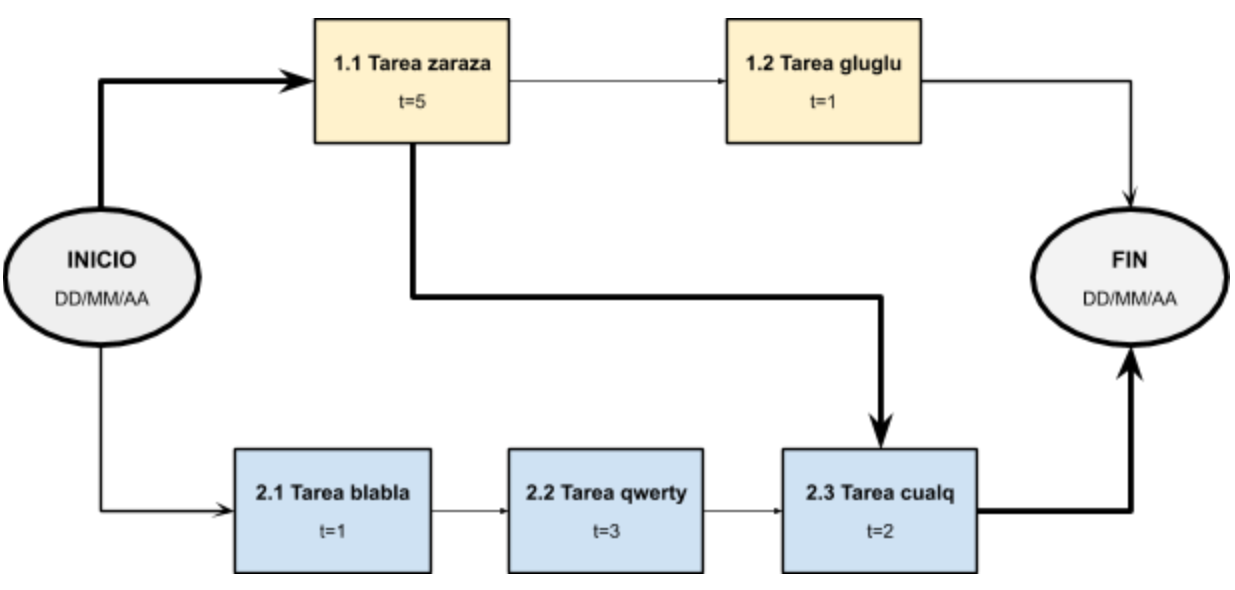
\includegraphics[width=.8\textwidth]{./fig/AoN.png}
\caption{Diagrama en \textit{Activity on Node}}
\label{fig:AoN}
\end{figure}

Indicar claramente en qué unidades están expresados los tiempos.
De ser necesario indicar los caminos semicríticos y analizar sus tiempos mediante un cuadro.
Es recomendable usar colores y un cuadro indicativo describiendo qué representa cada color, como se muestra en el siguiente ejemplo:



\section{11. Diagrama de Gantt}
\label{sec:gantt}

\begin{consigna}{red}

Existen muchos programas y recursos \textit{online} para hacer diagramas de gantt, entre los cuales destacamos:

\begin{itemize}
\item Planner
\item GanttProject
\item Trello + \textit{plugins}. En el siguiente link hay un tutorial oficial: \\ \url{https://blog.trello.com/es/diagrama-de-gantt-de-un-proyecto}
\item Creately, herramienta online colaborativa. \\\url{https://creately.com/diagram/example/ieb3p3ml/LaTeX}
\item Se puede hacer en latex con el paquete \textit{pgfgantt}\\ \url{http://ctan.dcc.uchile.cl/graphics/pgf/contrib/pgfgantt/pgfgantt.pdf}
\end{itemize}

Pegar acá una captura de pantalla del diagrama de Gantt, cuidando que la letra sea suficientemente grande como para ser legible. 
Si el diagrama queda demasiado ancho, se puede pegar primero la ``tabla'' del Gantt y luego pegar la parte del diagrama de barras del diagrama de Gantt.

Configurar el software para que en la parte de la tabla muestre los códigos del EDT (WBS).\\
Configurar el software para que al lado de cada barra muestre el nombre de cada tarea.\\
Revisar que la fecha de finalización coincida con lo indicado en el Acta Constitutiva.

En la figura \ref{fig:gantt}, se muestra un ejemplo de diagrama de gantt realizado con el paquete de \textit{pgfgantt}. En la plantilla pueden ver el código que lo genera y usarlo de base para construir el propio.

\begin{figure}[htbp]
\begin{center}
\begin{ganttchart}{1}{12}
  \gantttitle{2020}{12} \\
  \gantttitlelist{1,...,12}{1} \\
  \ganttgroup{Group 1}{1}{7} \\
  \ganttbar{Task 1}{1}{2} \\
  \ganttlinkedbar{Task 2}{3}{7} \ganttnewline
  \ganttmilestone{Milestone o hito}{7} \ganttnewline
  \ganttbar{Final Task}{8}{12}
  \ganttlink{elem2}{elem3}
  \ganttlink{elem3}{elem4}
\end{ganttchart}
\end{center}
\caption{Diagrama de gantt de ejemplo}
\label{fig:gantt}
\end{figure}


\begin{landscape}
\begin{figure}[htpb]
\centering 
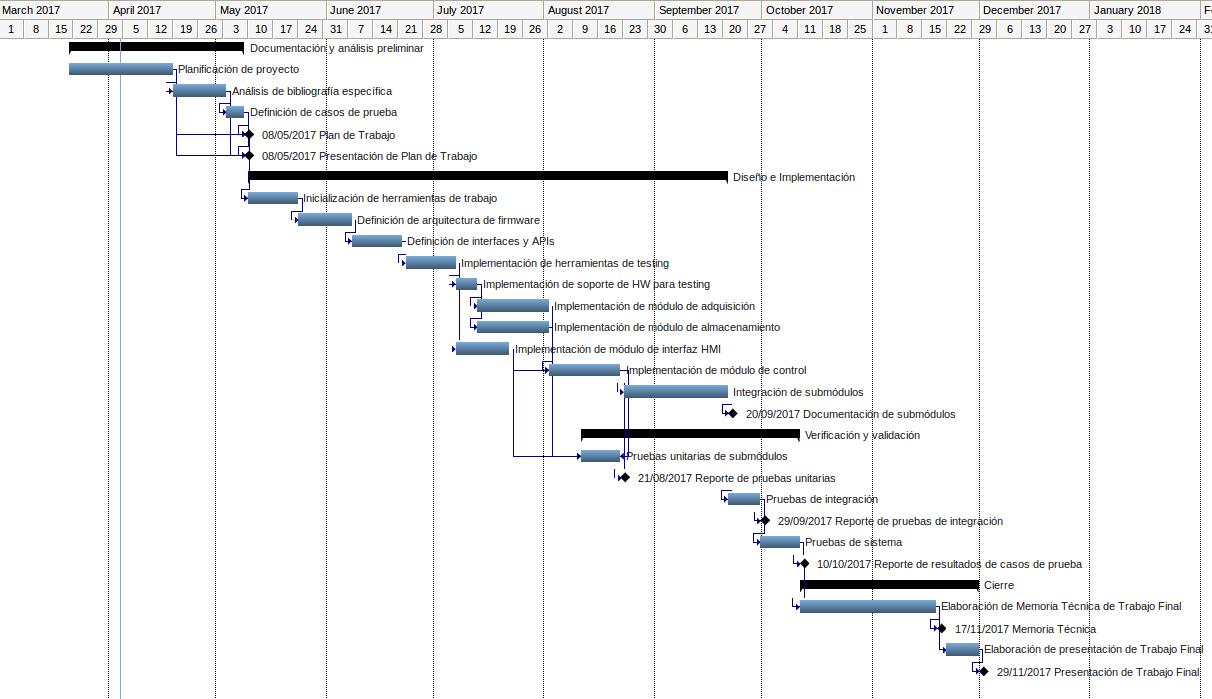
\includegraphics[height=.85\textheight]{./fig/Gantt-2.png}
\caption{Ejemplo de diagrama de Gantt rotado}
\label{fig:diagGantt}
\end{figure}

\end{landscape}

\end{consigna}


\section{12. Presupuesto detallado del proyecto}
\label{sec:presupuesto}

\begin{consigna}{red}
Si el proyecto es complejo entonces separarlo en partes:
\begin{itemize}
	\item Un total global, indicando el subtotal acumulado por cada una de las áreas.
	\item El desglose detallado del subtotal de cada una de las áreas.
\end{itemize}

IMPORTANTE: No olvidarse de considerar los COSTOS INDIRECTOS.

\end{consigna}

\begin{table}[htpb]
\centering
\begin{tabularx}{\linewidth}{@{}|X|c|r|r|@{}}
\hline
\rowcolor[HTML]{C0C0C0} 
\multicolumn{4}{|c|}{\cellcolor[HTML]{C0C0C0}COSTOS DIRECTOS} \\ \hline
\rowcolor[HTML]{C0C0C0} 
Descripción &
  \multicolumn{1}{c|}{\cellcolor[HTML]{C0C0C0}Cantidad} &
  \multicolumn{1}{c|}{\cellcolor[HTML]{C0C0C0}Valor unitario} &
  \multicolumn{1}{c|}{\cellcolor[HTML]{C0C0C0}Valor total} \\ \hline
 &
  \multicolumn{1}{c|}{} &
  \multicolumn{1}{c|}{} &
  \multicolumn{1}{c|}{} \\ \hline
 &
  \multicolumn{1}{c|}{} &
  \multicolumn{1}{c|}{} &
  \multicolumn{1}{c|}{} \\ \hline
\multicolumn{1}{|l|}{} &
   &
   &
   \\ \hline
\multicolumn{1}{|l|}{} &
   &
   &
   \\ \hline
\multicolumn{3}{|c|}{SUBTOTAL} &
  \multicolumn{1}{c|}{} \\ \hline
\rowcolor[HTML]{C0C0C0} 
\multicolumn{4}{|c|}{\cellcolor[HTML]{C0C0C0}COSTOS INDIRECTOS} \\ \hline
\rowcolor[HTML]{C0C0C0} 
Descripción &
  \multicolumn{1}{c|}{\cellcolor[HTML]{C0C0C0}Cantidad} &
  \multicolumn{1}{c|}{\cellcolor[HTML]{C0C0C0}Valor unitario} &
  \multicolumn{1}{c|}{\cellcolor[HTML]{C0C0C0}Valor total} \\ \hline
\multicolumn{1}{|l|}{} &
   &
   &
   \\ \hline
\multicolumn{1}{|l|}{} &
   &
   &
   \\ \hline
\multicolumn{1}{|l|}{} &
   &
   &
   \\ \hline
\multicolumn{3}{|c|}{SUBTOTAL} &
  \multicolumn{1}{c|}{} \\ \hline
\rowcolor[HTML]{C0C0C0}
\multicolumn{3}{|c|}{TOTAL} &
   \\ \hline
\end{tabularx}%
\end{table}


\section{13. Gestión de riesgos}
\label{sec:riesgos}

\begin{consigna}{red}
a) Identificación de los riesgos (al menos cinco) y estimación de sus consecuencias:
 
Riesgo 1: detallar el riesgo (riesgo es algo que si ocurre altera los planes previstos de forma negativa)
\begin{itemize}
	\item Severidad (S): mientras más severo, más alto es el número (usar números del 1 al 10).\\
	Justificar el motivo por el cual se asigna determinado número de severidad (S).
	\item Probabilidad de ocurrencia (O): mientras más probable, más alto es el número (usar del 1 al 10).\\
	Justificar el motivo por el cual se asigna determinado número de (O). 
\end{itemize}   

Riesgo 2:
\begin{itemize}
	\item Severidad (S): 
	\item Ocurrencia (O):
\end{itemize}

Riesgo 3:
\begin{itemize}
	\item Severidad (S): 
	\item Ocurrencia (O):
\end{itemize}


b) Tabla de gestión de riesgos:      (El RPN se calcula como RPN=SxO)

\begin{table}[htpb]
\centering
\begin{tabularx}{\linewidth}{@{}|X|c|c|c|c|c|c|@{}}
\hline
\rowcolor[HTML]{C0C0C0} 
Riesgo & S & O & RPN & S* & O* & RPN* \\ \hline
       &   &   &     &    &    &      \\ \hline
       &   &   &     &    &    &      \\ \hline
       &   &   &     &    &    &      \\ \hline
       &   &   &     &    &    &      \\ \hline
       &   &   &     &    &    &      \\ \hline
\end{tabularx}%
\end{table}

Criterio adoptado: 
Se tomarán medidas de mitigación en los riesgos cuyos números de RPN sean mayores a...

Nota: los valores marcados con (*) en la tabla corresponden luego de haber aplicado la mitigación.

c) Plan de mitigación de los riesgos que originalmente excedían el RPN máximo establecido:
 
Riesgo 1: plan de mitigación (si por el RPN fuera necesario elaborar un plan de mitigación).
  Nueva asignación de S y O, con su respectiva justificación:
  - Severidad (S): mientras más severo, más alto es el número (usar números del 1 al 10).
          Justificar el motivo por el cual se asigna determinado número de severidad (S).
  - Probabilidad de ocurrencia (O): mientras más probable, más alto es el número (usar del 1 al 10).
          Justificar el motivo por el cual se asigna determinado número de (O).

Riesgo 2: plan de mitigación (si por el RPN fuera necesario elaborar un plan de mitigación).
 
Riesgo 3: plan de mitigación (si por el RPN fuera necesario elaborar un plan de mitigación).

\end{consigna}


\section{14. Gestión de la calidad}
\label{sec:calidad}

\begin{consigna}{red}
Para cada uno de los requerimientos del proyecto indique:
\begin{itemize} 
\item Req \#1: copiar acá el requerimiento.

\begin{itemize}
	\item Verificación para confirmar si se cumplió con lo requerido antes de mostrar el sistema al cliente. Detallar 
	\item Validación con el cliente para confirmar que está de acuerdo en que se cumplió con lo requerido. Detallar  
\end{itemize}

\end{itemize}

Tener en cuenta que en este contexto se pueden mencionar simulaciones, cálculos, revisión de hojas de datos, consulta con expertos, mediciones, etc.  Las acciones de verificación suelen considerar al entregable como ``caja blanca'', es decir se conoce en profundidad su funcionamiento interno.  En cambio, las acciones de validación suelen considerar al entregable como ``caja negra'', es decir, que no se conocen los detalles de su funcionamiento interno.

\end{consigna}

\section{15. Procesos de cierre}    
\label{sec:cierre}

\begin{consigna}{red}
Establecer las pautas de trabajo para realizar una reunión final de evaluación del proyecto, tal que contemple las siguientes actividades:

\begin{itemize}
	\item Pautas de trabajo que se seguirán para analizar si se respetó el Plan de Proyecto original:
	 - Indicar quién se ocupará de hacer esto y cuál será el procedimiento a aplicar. 
	\item Identificación de las técnicas y procedimientos útiles e inútiles que se emplearon, y los problemas que surgieron y cómo se solucionaron:
	 - Indicar quién se ocupará de hacer esto y cuál será el procedimiento para dejar registro.
	\item Indicar quién organizará el acto de agradecimiento a todos los interesados, y en especial al equipo de trabajo y colaboradores:
	  - Indicar esto y quién financiará los gastos correspondientes.
\end{itemize}

\end{consigna}


\end{document}
